\subsection{Noradrenerges System}
\label{noradrenerges_system}
%%%%%%%%%%%%%%%%%%%%%%%%%%%%%%%%%%
\index{System! noradrenerg}
Genau wie Dopamin gehört auch Noradrenalin\index{Noradrenalin} (engl.: Norepinephrine, Abb.~\ref{fig:noradrenalin}) zu den Catecholaminen \textsuperscript{\cite[Kap.~1]{trepel2011neuroanatomie}}. Das Enzym Dopamin-$\upbeta$-Hydroxylase wandelt Dopamin zu Noradrenalin um. Durch die Phenylethanolamin-N-Methyltransferase wird Noradrenalin zu Adrenalin (engl.: Epinephrin) umgewandelt \textsuperscript{\cite[Kap.~13]{kandel2013principles}}. Noradrenalin kommt als Transmitter sowohl im zentralen als auch im sympathischen, peripheren Nervensystem vor \textsuperscript{\cite[Kap.~4]{crossman2014neuroanatomy}}. Innerhalb des zentralen Nervensystem wird Noradrenalin im Hirnstamm, in der Formatio reticularis, synthetisiert \textsuperscript{\cite[Kap.~7]{trepel2011neuroanatomie}}.

\begin{figure}[H]
    \centering
    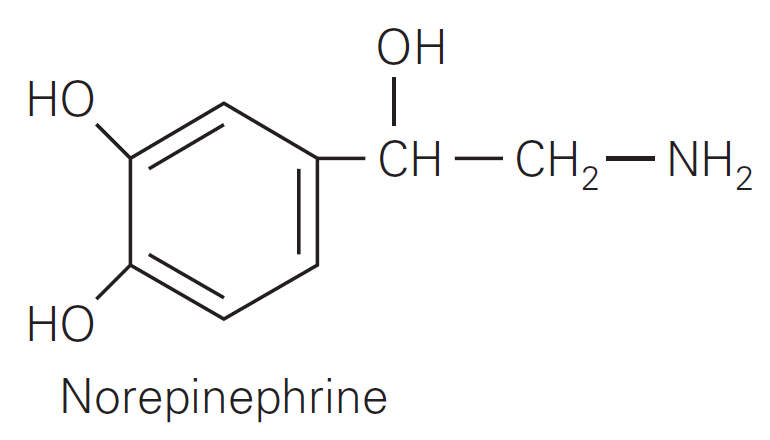
\includegraphics[width=0.4\textwidth]{pictures/Bilder_monoamine_systeme/noradrenalin.PNG}
    \caption[Noradrenalin]{\textbf{Noradrenalin.} Abbildung aus \textit{Principles of Neural Systems}, Kandel et al. \textsuperscript{\cite[Kap.~13]{kandel2013principles}}.}
    \label{fig:noradrenalin}
\end{figure}

Noradrenerge Neurone sind in kleineren Gebieten des Pons und der Medulla zu finden \textsuperscript{\cite[Kap.~24]{kandel2013principles}}. Der \textit{Locus coeruleus}\index{Locus coeruleus} (Abb.~\ref{fig:locus_coeruleus}) wird aus absteigenden, noradrenergen Fasern im oberen Pons gebildet. Seine pigmentierten Neurone sind im rostralen pontinen Tegmentum lokalisiert \textsuperscript{\cite[Kap.~8]{crossman2014neuroanatomy}}. Die dort entspringenden, überwiegenden inhibitorischen Projektionen sind im zentralen Nervensystem weit verstreut \textsuperscript{\cite[Kap.~6]{trepel2011neuroanatomie}}. Sie projizieren ins Cerebellum, in den Hirnstamm und das Rückenmark, aber auch in viele Teilbereiche des Vorderhirns (Proencephalon). Dazu gehören das Diencephalon, limbische Strukturen und der cerebrale Cortex (Abb.~\ref{noradrenerges_system}). Die noradrenerge Innervation des Proencephalons kann mit höheren kognitiven Funktionen und Gemütszuständen in Verbindung gebracht werden \textsuperscript{\cite[Kap.~8]{crossman2014neuroanatomy}}.

\begin{figure}[H]
    \centering
    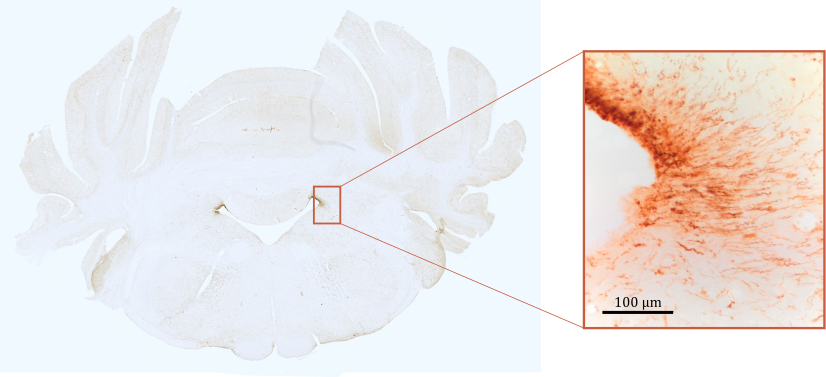
\includegraphics[width=\textwidth]{pictures/Bilder_monoamine_systeme/locus_coeruleus.png}
    \caption[Locus coeruleus]{\textbf{Locus coeruleus.} Dargestellt sind die noradrenergen Neurone des Locus coeruleus, die im Pons lokalisiert sind (Ia04-3). Neben den angefärbten Neuronen des Locus coeruleus (rechts) sind auch der vierte Ventrikel (\textbf{4V}), das Cerebellum (\textbf{Cb}) und der Pyramidentrakt (\textbf{py}) zu sehen.}
    \label{fig:locus_coeruleus}
\end{figure}

Funktionell spielten die noradrenergen Neurone des Locus coeruleus eine wichtige Rolle in Aufmerksamkeitszuständen \textsuperscript{\cite[Kap.~46]{kandel2013principles}}. Gemeinsam mit dem aufsteigenden retikulären Aktivierungssystem (ARAS) ist er an der Entstehung des Schlaf-Wach-Rhythmus beteiligt. Zudem wird der Locus coeruleus in körperlichen und seelischen Stresssituationen aktiviert und wirkt somit als eine Art 'Alarmsystem des Gehirns'. Er ist an der Entstehung von Angstempfindung und Herzrasen (Tachykardie) beteiligt. Fehlfunktionen der noradrenergen Projektionen in Bereiche des limbischen Systems können zudem mit Depression, Schlafstörungen und dem Hyperaktivitätssyndrom in Verbindung gebracht werden \textsuperscript{\cite[Kap.~6]{trepel2011neuroanatomie}}.

\begin{figure}[H]
    \centering
    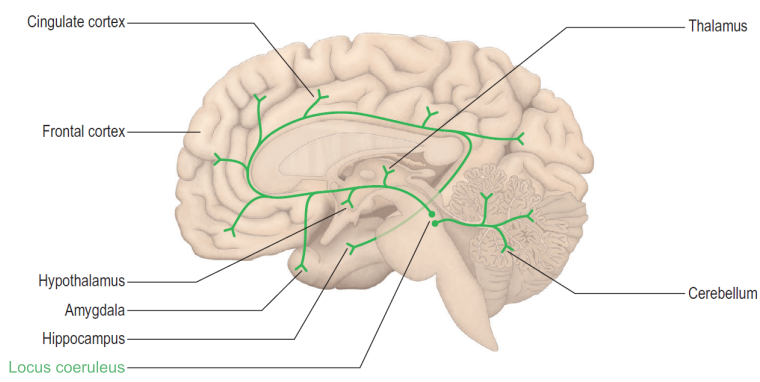
\includegraphics[width=\textwidth]{pictures/Bilder_monoamine_systeme/noradrenerges_system.PNG}
    \caption[Noradrenerges System]{\textbf{Noradrenerges System.} Noradrenerge Neurone sind in der Medulla und im Pons lokalisiert. Der Locus coeruleus des Pons ist das wichtigste noradrenerge Kerngebiet. Abbildung nach \textit{Neuroanatomy}, Crossman und Neary \textsuperscript{\cite[Kap.~9]{crossman2014neuroanatomy}}.}
    \label{fig:noradrenerges_system}
\end{figure}{}

